\section{Authoritative-state admission contract}
\label{sec:contract}

\subsection{Mutation is not admission}

Authorized mutation begins with an object $o_v$ that is already authoritative and applies an authorized change $\alpha$:
\begin{equation}
\operatorname{Mutate}(o_v,\alpha)=o_{v+1}.
\end{equation}
Correction-aware admission begins instead with an untrusted persisted candidate $c$, an attributable authorization $a$, and an authoritative pre-state $S_v$:
\begin{equation}
\operatorname{Admit}(c,a,S_v)=S_{v+1}.
\label{eq:admit}
\end{equation}
Admission does not make the candidate itself authoritative. It transforms a candidate-bound authorization into an authoritative successor while retaining the candidate as non-authoritative historical evidence. Proposal origin, value authority, and committed value are therefore distinct semantic roles.

Let $r$ be a record with a nonempty authoritative field set $F_r$. A committed version $v$ contains a total value map $V_v:F_r\rightarrow X$ and a total source map $S_v:F_r\rightarrow T$, where $T$ is the set of durable fact transitions. A machine candidate for field $f$ is
\begin{equation}
c=\langle r,f,e,v_{\mathrm{exp}},x_c,p,c_{\mathrm{id}}\rangle,
\label{eq:candidate}
\end{equation}
where $e$ is persisted evidence, $v_{\mathrm{exp}}$ is the expected current version, $x_c$ is the machine proposal, $p$ identifies its producer, and $c_{\mathrm{id}}$ is an identity over the modeled candidate content.

Evidence identity is not content equality alone. The realization uses
\begin{equation}
EID(e)=\langle H(\mathrm{bytes}(e)),L(r,f,u,\kappa)\rangle,
\label{eq:evidence}
\end{equation}
where $H$ is SHA-256 and $L$ is a versioned canonical locator containing the owner record, related field, normalized storage-relative URI $u$, and optional crop identity $\kappa$. The formal model treats content and locator as primitive domains and does not assume that SHA-256 is injective.

An attributable authorization is
\begin{equation}
a=\langle c_{\mathrm{id}},x_a,q\rangle,
\label{eq:authorization}
\end{equation}
where $q$ is an authorized human principal and $x_a$ is the value explicitly permitted to enter the record. The dual-value semantics are
\begin{align}
\operatorname{proposal}(c)&=x_c, &
\operatorname{authorize}(a)&=x_a,\nonumber\\
\operatorname{commit}(S_{v+1},f)&=x_a, &
\operatorname{origin}(S_{v+1},f)&=c.
\label{eq:dual-value}
\end{align}
Accept has $x_c=x_a$. Correction has $x_c\neq x_a$; the candidate remains unchanged and the committed value derives its authority from $a$.

\subsection{History, observations, and outcomes}

An authority-relevant history is
\begin{equation}
h=S_0\xrightarrow{e_1}S_1\xrightarrow{e_2}\cdots\xrightarrow{e_n}S_n,
\end{equation}
where events may persist evidence or candidates, record review and authorization, attempt admission, commit or stutter, and reconstruct a reverse trace. The abstraction describes semantic information rather than requiring particular table or column names.

We group the observable distinctions into
\begin{equation}
\mathcal D=\{D_C,D_V,D_F,D_B,D_S\},
\label{eq:distinction-basis}
\end{equation}
where $D_C$ is candidate identity and context, $D_V$ is dual-value attribution, $D_F$ is freshness, $D_B$ is batch/successor completeness, and $D_S$ is total source attribution. For $I\subseteq\mathcal D$, $\pi_I(h)$ retains only the information classes in $I$. Candidate identity may be implemented by a certificate, stable handle, or another equivalence class, provided it does not collapse to value equality. Freshness may likewise use a version, state hash, epoch, or comparable discriminator.

The observable authority outcome is
\begin{equation}
O(h)=\langle status,successor,trace\rangle,
\label{eq:outcome}
\end{equation}
where $status$ is accept, reject, or failed/stuttering attempt; $successor$ is the authoritative post-state or absence of one; and $trace$ is complete, incomplete, ambiguous, or unavailable. A binary accept/reject outcome is insufficient because value-identical successors may differ in source completeness.

An observation set $I$ fails to distinguish a failure family when there exist a safe history $h_s$ and unsafe history $h_u$ such that
\begin{equation}
O(h_s)\neq O(h_u)
\quad\land\quad
\pi_I(h_s)=\pi_I(h_u).
\label{eq:indistinguishable}
\end{equation}
Any admission decision based only on that reduced observation cannot separate the pair.

\subsection{Conditional failure-distinguishability characterization}

Table~\ref{tab:distinctions} states the five information classes of the declared basis. Each concerns an information class, not a mandatory physical representation.

\begin{table*}[t]
\centering
\footnotesize
\caption{Failure-distinguishing information classes in the declared observation model.}
\label{tab:distinctions}
\begin{tabularx}{\textwidth}{@{}l>{\raggedright\arraybackslash}p{0.23\textwidth}>{\raggedright\arraybackslash}p{0.27\textwidth}>{\raggedright\arraybackslash}X@{}}
\toprule
Class & Safe/unsafe pair & Required distinction & Failure if omitted \\
\midrule
$D_C$ & exact candidate / equal-valued cross-context substitute & persisted candidate identity plus record, field, evidence, and producer context & candidate substitution \\
$D_V$ & preserved Correction / rewritten or erased proposal & separate machine proposal $x_c$, human-authorized value $x_a$, and role relation & correction erasure or false machine attribution \\
$D_F$ & current authorization / same authorization after supersession & commit-time freshness discriminator tied to the observed pre-state & stale replay \\
$D_B$ & complete batch / subset of declared field effects & declared batch domain, exact changed-field framing, and one atomic successor & partial successor \\
$D_S$ & total trace / equal-valued successor with missing or conflicting source & total per-field source relation and exact unchanged-source copy-forward & source ambiguity \\
\bottomrule
\end{tabularx}
\end{table*}

\paragraph{Proposition 1 (conditional failure distinguishability).}
For each information class $d_i\in\mathcal D$, the declared failure model contains a safe history and a corresponding unsafe history whose authority outcomes differ but whose projections become equal when $d_i$ is omitted. Consequently, an admission mechanism that observes only $\mathcal D\setminus\{d_i\}$ cannot distinguish the paired failure family under this model.

\paragraph{Proof sketch (by construction).}
For each declared failure family associated with $d_i\in\mathcal D$, Table~\ref{tab:distinctions} provides a paired construction consisting of a safe history $h_s^{(i)}$ and an unsafe history $h_u^{(i)}$ such that
$O(h_s^{(i)})\neq O(h_u^{(i)})$ while
$\pi_{\mathcal D\setminus\{d_i\}}(h_s^{(i)})=\pi_{\mathcal D\setminus\{d_i\}}(h_u^{(i)})$.
The five constructions are as follows. For $D_C$, hold value and authorization payload constant but substitute a candidate from another record, field, or evidence object. For $D_V$, hold the final value constant but compare a history retaining both 100 and a human-authorized 101 with one that rewrites the machine proposal as 101. For $D_F$, replay the same candidate and authorization bytes before and after another transaction advances the record. For $D_B$, hold the visible values of one affected field constant while omitting another declared batch effect. For $D_S$, hold every successor value constant while deleting, replacing, or duplicating a field source. In each construction, removing the paired class makes the safe and unsafe projections equal although their intended outcomes differ.

Formally, for each $d_i\in\mathcal D$, the construction seeks histories $h_s^{(i)}$ and $h_u^{(i)}$ such that
\begin{equation}
\pi_{\mathcal D\setminus\{d_i\}}(h_s^{(i)})
=
\pi_{\mathcal D\setminus\{d_i\}}(h_u^{(i)})
\quad\text{and}\quad
O(h_s^{(i)})\neq O(h_u^{(i)}).
\label{eq:irredundancy}
\end{equation}
Therefore, removing the corresponding information class eliminates the ability to distinguish at least one declared failure family.

\paragraph{Scope of the result.}
Proposition 1 establishes class-wise irredundancy relative to the five declared failure families and the declared history, observation, and outcome model. It does not establish universal minimality, schema uniqueness, or completeness over all possible admission failures. The Full Alloy checks provide sufficiency-like evidence only in the encoded finite scopes; the ablations provide bounded witnesses for selected encodings of the five classes.

\subsection{Batch admission relation}

A batch $B$ is a nonempty set of items sharing one target record, principal, expected pre-version, and successor. Under Full, item fields are unique. Let
\begin{equation}
\Delta(V_v,V_{v+1})=\{f\in F_r\mid V_v(f)\neq V_{v+1}(f)\}.
\end{equation}
For a post-initial concrete admission,
\begin{equation}
\Delta(V_v,V_{v+1})=\{i.f\mid i\in B\}=\{t.f\mid t\in T_{v+1}\},
\label{eq:changed-fields}
\end{equation}
with one transition per item. At the first certificate-era version, the batch covers all of $F_r$, establishing total value and source domains. Deletion is outside the model.

For every $i\in B$, admission requires
\begin{align}
i.r &= r, & i.f&\in F_r,\nonumber\\
EID(i.e) &= EID(i.c.e), & i.v_{\mathrm{exp}}&=v,\nonumber\\
i.a.c_{\mathrm{id}}&=i.c.c_{\mathrm{id}}, & i.a.q&=q,\nonumber\\
i.x&=i.a.x_a, & t_i.x&=V_{v+1}(i.f)=i.x.
\label{eq:item-bindings}
\end{align}
Together these instantiate the admission preconditions
\begin{equation}
\operatorname{Bind}(a,c)\land\operatorname{Fresh}(c,S_v)\land
\operatorname{Authorized}(a)\land\operatorname{Complete}(S_{v+1})\land
\operatorname{Attributed}(S_{v+1}).
\end{equation}

The successor is atomic: either all decision, authorization, transition, version, source-map, and audit effects commit, or authoritative state stutters. For a changed field, $S_{v+1}(f)=t_i$. For an unchanged field, both value and exact source are copied forward:
\begin{equation}
f\notin\Delta(V_v,V_{v+1})\Rightarrow
V_{v+1}(f)=V_v(f)\land S_{v+1}(f)=S_v(f).
\label{eq:copy-forward}
\end{equation}
The Alloy relation permits same-value admission for correspondence with the historical singleton model. The concrete service rejects a post-initial batch with an empty changed-field set; accepted concrete events are therefore a strict value-changing subset of formal legal events.

\subsection{Operational properties and trust boundary}

\begin{table*}[t]
\centering
\caption{Locked properties and their operational interpretation.}
\label{tab:properties}
\begin{tabularx}{\textwidth}{@{}l>{\raggedright\arraybackslash}p{0.29\textwidth}>{\raggedright\arraybackslash}X@{}}
\toprule
Property & Requirement & Operational interpretation \\
\midrule
P0 & Direct-write exclusion & Machine/candidate capability cannot change authoritative values, versions, sources, transitions, or authorizations. \\
P1 & Candidate non-substitutability & Authority refers to the same canonical persisted certificate, not merely an equal value or analogous candidate. \\
P2 & Context-bound admission & Record, field, persisted evidence content and locator, and expected version agree across the item and certificate. \\
P3 & Authorization integrity & The principal is allowed at commit and the authorization names the exact certificate and explicit committed value. \\
P4 & Freshness & The expected version equals the transactionally observed current version; stale or competing decisions fail closed. \\
P5 & Successor integrity & One atomic successor has an item--transition bijection, exact changed-field effects, and complete changed/unchanged framing. \\
P6 & Trace soundness & Each committed field resolves through its exact source transition to consistent authorization, certificate, evidence, producer, and version relations. \\
\bottomrule
\end{tabularx}
\end{table*}

The untrusted side includes model output and callers possessing only candidate-write capability. The trusted computing base includes the admission service, narrow database adapter, SQLite transaction semantics for the exercised configuration, canonical serialization and hashing, and principal-policy source. Host authentication and session integrity are external assumptions: the prototype rechecks whether a supplied principal is active and has an allowed role, but it does not authenticate a human or protect a compromised process, host, or database administrator.

Human authorization is not a truth oracle. The contract establishes who authorized which persisted candidate and value in which context, and whether the successor was constructed atomically. It cannot establish that the authorized value is factually correct.

\Cref{fig:admission-workflow} summarizes the capability boundary and trusted transaction.

% FIGURE SOURCE: exact author-approved Canva design DAHUNAr-imw export. The PDF is the manuscript source; a matching converted SVG is retained beside it for downstream reuse.
\begin{figure*}[t]
\centering
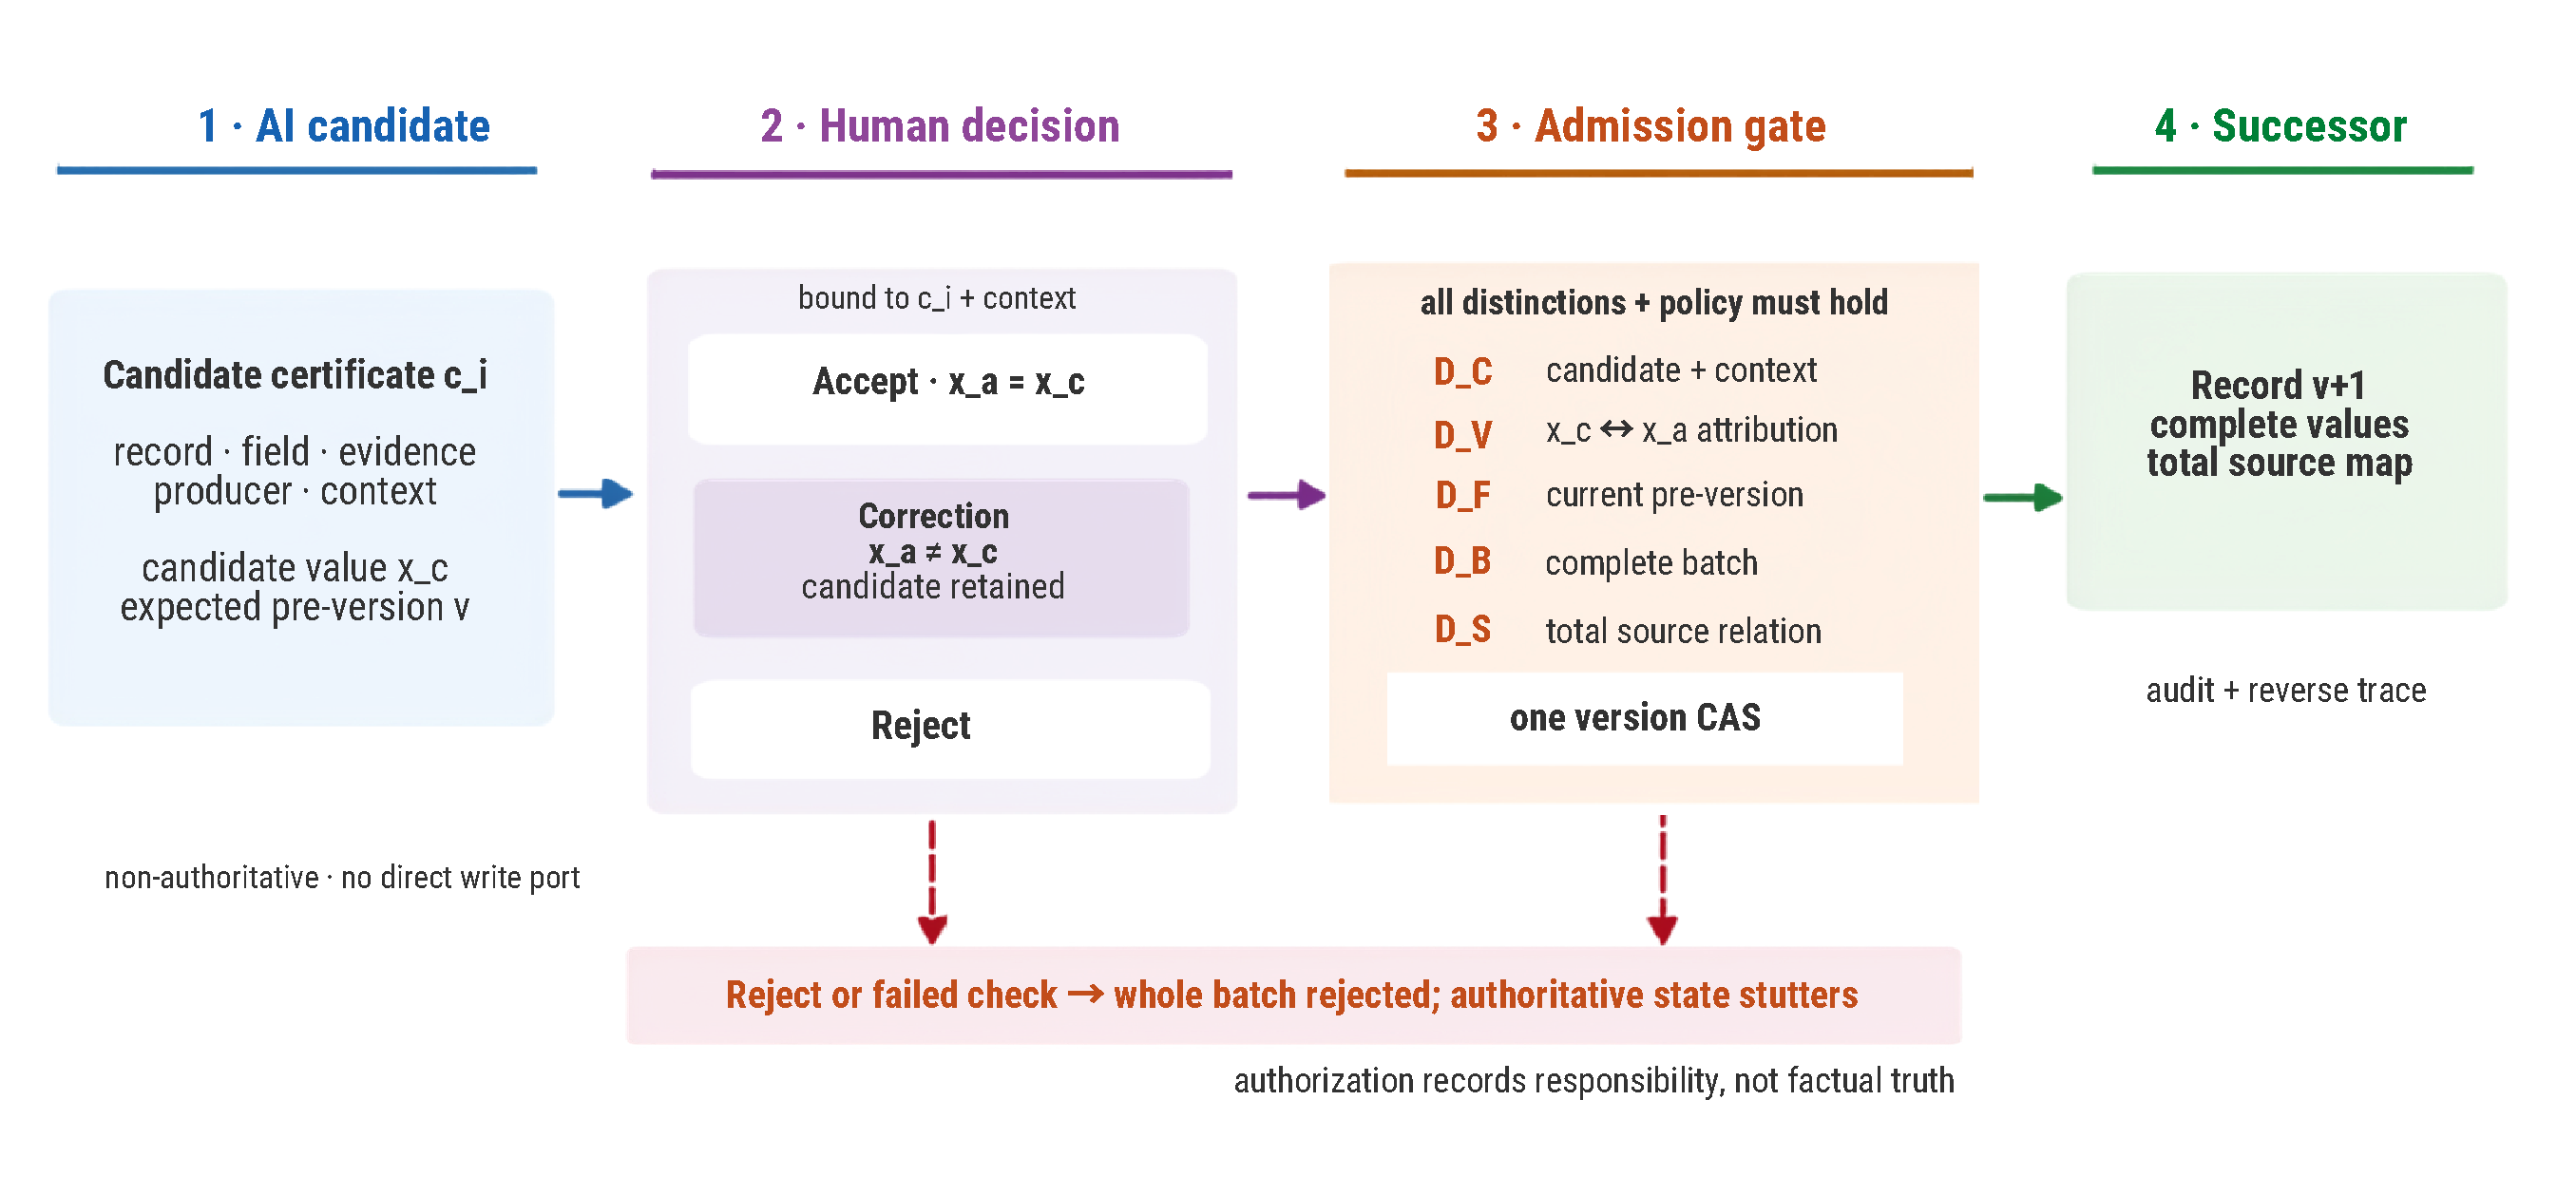
\includegraphics[width=0.96\textwidth]{figures/canva/admission-workflow-canva.pdf}
\caption{Correction-aware authoritative-state admission. A persisted AI candidate has no direct authoritative write port. A candidate-bound human decision may Accept the proposed value, Correct it while retaining the exact candidate, or Reject it. Admission succeeds only when the five distinction classes and principal policy hold; one version compare-and-swap then creates a complete successor and total source map. Reject or failed validation leaves the authoritative state unchanged.}
\label{fig:admission-workflow}
\end{figure*}
